\subsection{Datenstruktur}
Die Datenstruktur der Anwendung besteht grundsätzlich aus drei abstrakten und fünf konkreten Klassen. Die abstrakten Klassen sind Entitäten, organisationsbasierende Entitäten und verlinkbare Entitäten. Die absoluten Klassen sind Nutzer, Organisation, Level, Gruppe und Aufgabe.

\vspace{20pt}
\begin{center}
    \begin{minipage}{1\linewidth}
        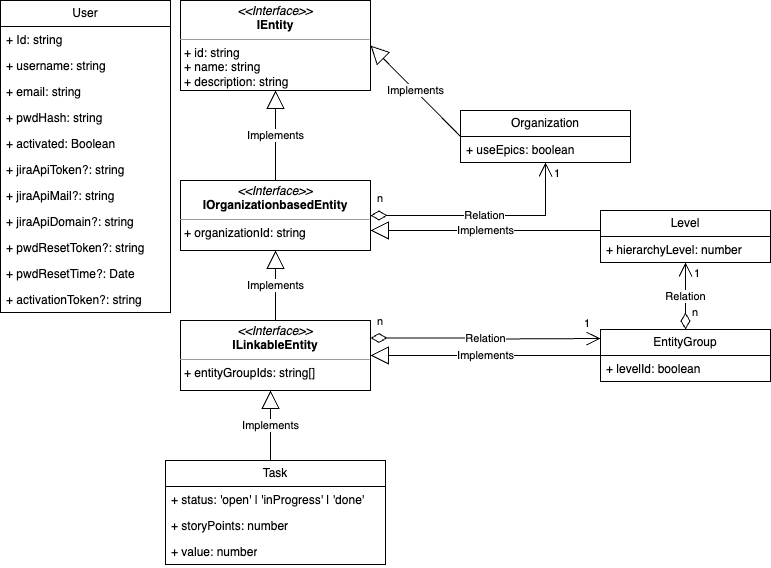
\includegraphics[width=\linewidth]{classDiagramm}
        \captionof{figure}{UML-Diagramm der Datenstruktur}
    \end{minipage}
\end{center}
\vspace{20pt}

Jede absolute Klasse, außer die Nutzer, erben von einer oder mehreren abstrakten Klassen. Entitäten sind allgemeine Objekte innerhalb der Anwendung und stellen die Grundlage der in der Datenbank gespeicherten Datenobjekte dar. Alle Klassen außer Nutzer sind solche Entitäten und implementieren das Interface \verb|IEntity|, welches eine ID zur eindeutigen Identifikation und einen Namen für die Darstellung für den Nutzer beinhaltet. Organisationen und Levels sind direkte Erben dieser Klasse. Die nächste Abstraktionsstufe sind die organisationsbasierenden Entitäten. Diese implementieren zu dem \verb|IEntity| Interface noch \verb|IOrganizationBasedEntity|, welches die ID einer Organisation voraussetzt und die Entität direkt von einer Organisation abhängig macht. Die letzte Abstraktionsstufe sind die verlinkbaren Entitäten. Diese implementieren zu dem \verb|IOrganizationBasedEntity| Interface noch \verb|ILinkableEntity|, welches eine Liste von IDs voraussetzt, mit dem gespeichert wird, mit welchen anderen verlinkbaren Entitäten das Objekt verlinkt ist. Aufgaben und Gruppen sind solche verlinkbare Entitäten.

\subsection{Backend-Architektur}
Das Backend ist eine REST-API, geschrieben mit Node.js und Express in TypeScript und verwendet mongoose als Datenbank-API für MongoDB. Die Architektur beschreibt die den Datenfluss mit drei allgemeinen Komponenten: Router, Controller und Service.
Der Router bestimmt für einen Request welche Funktion eines Controllers aufgerufen wird. Die aufgerufene Controller-Funktion beinhaltet die Business-Logik, die an den Request gebunden ist und führt diese aus. Um Daten aus der Datenbank zu holen oder die geholten Daten zu modifizieren gibt es für jede Datenklasse einen Service, der die benötigten Datenbankoperationen implementiert und somit von der Business-Logik trennt. Für die Interaktion mit der Datenbank muss außerdem ein sogenanntes Model definiert werden, welches die Beschreibung der Klasse also der Type in TypeScript mit der Datenbank-Collection und den Objekten darin verknüpft.

\vspace{20pt}
\begin{center}
    \begin{minipage}{1\linewidth}
        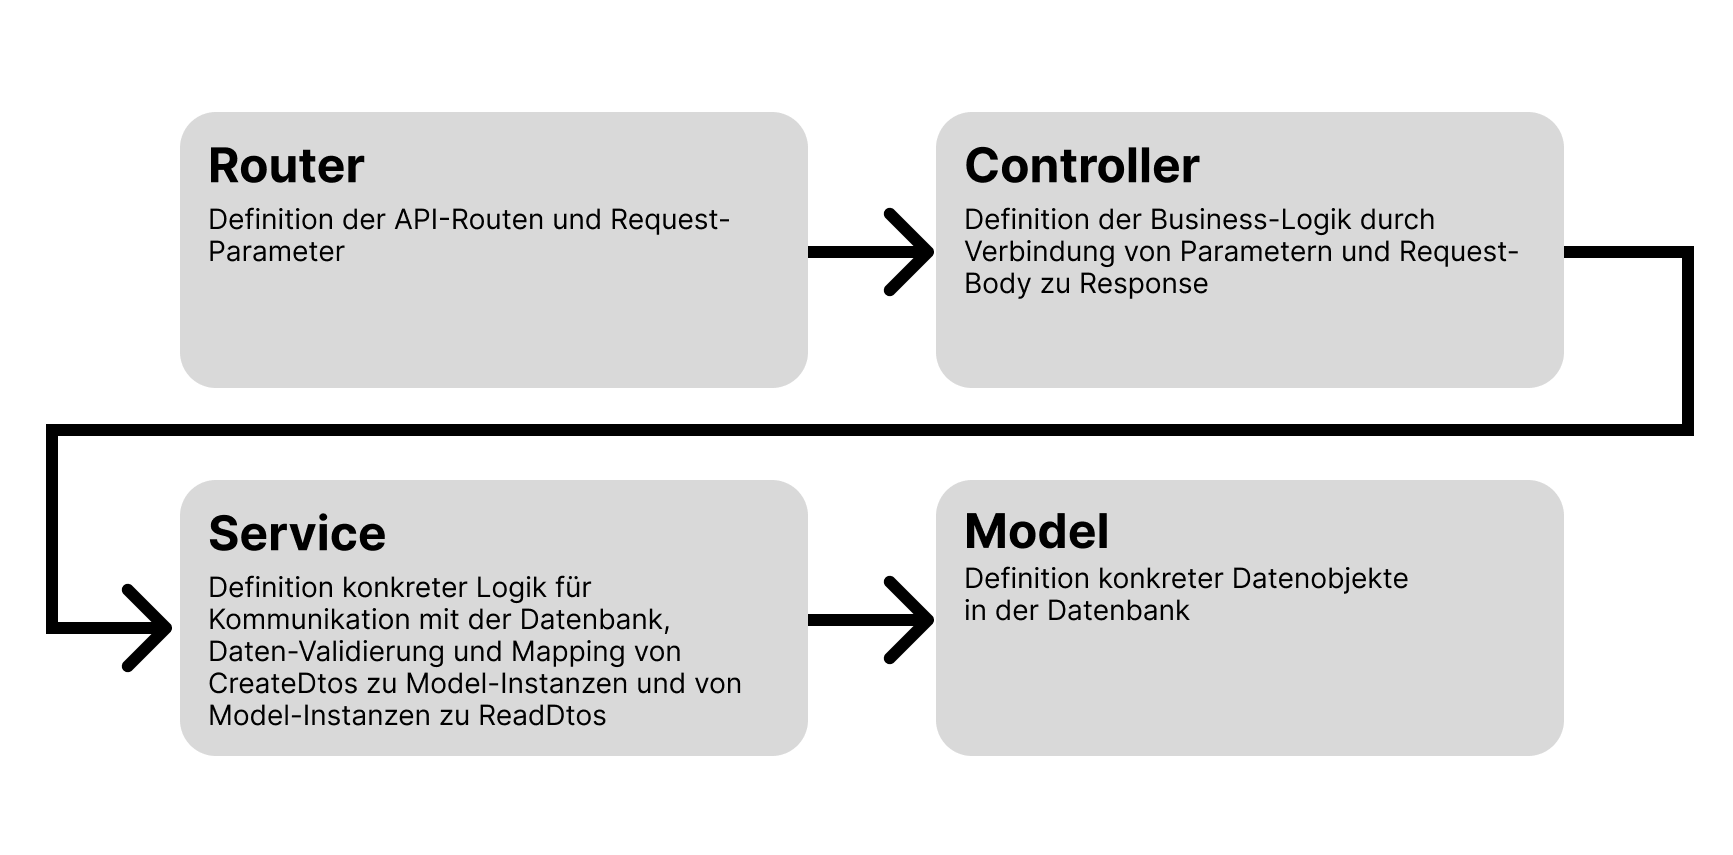
\includegraphics[width=\linewidth]{BE-Struktur}
        \captionof{figure}{Backend Architektur}
    \end{minipage}
\end{center}
\vspace{20pt}

Für die konkrete Kommunikation mit der REST-API werden zu den konkreten Datenobjekten innerhalb der Datenbank zwei weitere Klassen je Objekt-Klasse definiert. Diese Klassen sind sogenannte Data transfer Objects (DTO). DTOs dienen dazu die Kommunikation zu generalisieren und definieren die Daten die der Konsument der API durch einen Request erhalten kann und die Daten, die ein Konsument der API zur verfügung stellen kann, um z.B. ein neues Objekt in der Datenbank zu erstellen. Die zusätzlichen Klassendefinitionen werden durch diese zwei Anwendungsfälle in Read- und Create-/Update-DTOs unterteilt. Wie Create-/Update-DTOs zu einem internen Model gemappt werden und wie aus einem internen Model ein Read-Dto gemappt wird, definiert ebenfalls der zum Model zugehörige Service.

Der Aufbau des Backends gleicht dem Aufbau der Klassen-Abstraktion. Es gibt drei abstrakte Strukturen bestehend aus Router, Controller, Services und Model für jede der drei abstrakten Klassen und fünf absolute Strukturen für jede der fünf absoluten Klassen.


\vspace{20pt}
\begin{center}
    \begin{minipage}{1\linewidth}
        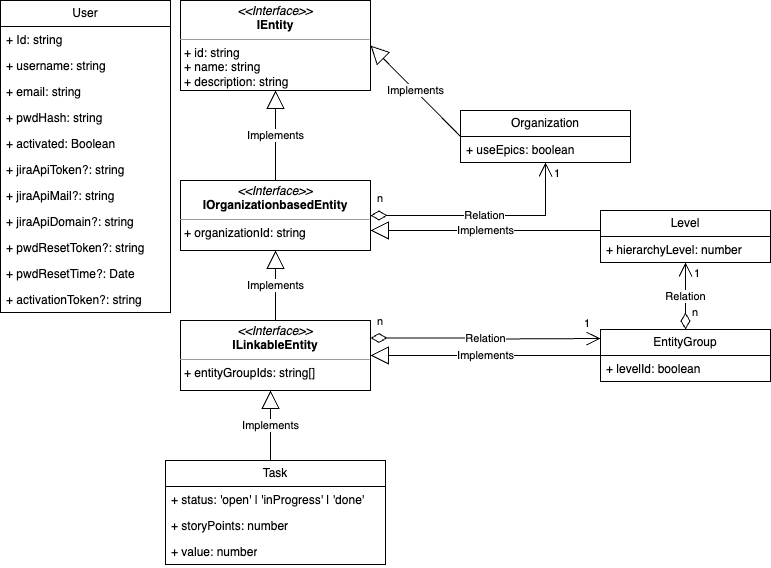
\includegraphics[width=\linewidth]{classDiagramm}
        \captionof{figure}{Abbildung der BE-Struktur}
    \end{minipage}
\end{center}
\vspace{20pt}

\emph{beschreibung de BE-Struktur}

\subsection{Benutzeroberfläche}
Zur initialen Planung wurde zunächst der UX-Entwurf verwendet um die grobe Struktur der Benutzeroberfläche zu entwickeln. Durch die spezifische Entwicklung verschiedener Features sind immer wieder Lücken im Entwurf aufgefallen und wurden duch weitere UI-Elemente erweitert um Funktionalitäten abzudecken, die zuvor nicht innerhalb des Prototypen bedacht wurden. Bis zum fertigen Prototypen haben sich viele der konkreten UI-Elemente verändert, allrdings blieb die Seitenstruktur also welche Informationen auf welches Seite dargestellt wurden identisch.

Für die Implementierung wurde als Frontend-/UI-Framework Vue.js verwendet. Vue.js ist eine Framwork für die Entwicklung von Single-Page-Webanwendungen. Es ist ein JavaScript-Framework, welches auf dem Model-View-ViewModel (MVVM) basiert. Die UI wurde also in verschiedene Komponenten zerteilt. Die Komponenten werden in zwei Kategorien unterteilt: Views und Components. Views sind logisch voneinander getrennte Seiten der Anwendung, während Components kleinere Bestandteile der Views zur vereinfachung der in der View benötigten Logik oder wiederverwendbare UI-Elemente sind. Zur weiteren Strukturierung werden hier noch sogenannte Layouts verwendet. Layouts stellen die Grundstruktur der Anwendung dar, welche von mehreren Views verwendet wird.

Die Anwendung teilt sich zunächst in zwei solcher Layouts: Authentifizierung und eigentliche Anwendung.

Das Layout der Authentifizierung beschreibt nur die Positionierung der relevanten Elemente in der Mitte des Bildschirms, da sich alle Seiten der Authentifizierung diese Eigenschaft teilen.
Das Layout der eigentlichen Seite teilt die Seite in drei Teile, den Header, den Inhalt und einen Footer. Der Header beinhaltet die Navigationsleiste, die den Nutzer durch die Anwendung führt und oben rechts ein Aktionsmenü mit dem der Nutzer sich jederzeit ausloggen kann oder in die Einstellungen bzw. sein Profil navigieren kann. Der Inhalt ist der Bereich in dem die verschiedenen Views dargestellt werden. Der Footer beinhaltet Informationen über den aktuell eingeloggten Nutzer.

\subsection{Visualisierung/Datendarstellung}


\subsection{CI/CD}
